\chapter{Related work}
\section{Object classification}
An example of object classification is whether, for a given image, if there is a cat or not in the image.

The most popular example of object classification is MNIST\cite{lecun-mnisthandwrittendigit-2010}, which was a task to find the number in the image (between 0 and 9).

Object classification is at the core of computer vision and it is probably the easiest task to solve.
This task could be used as an alternative to object detection though, because there isn't usually multiple animals anyway on the same picture and object classification is also faster since it doesn't have to infer location.

\pagebreak\subsection{Datasets}

\subsubsection{ImageNet}
ImageNet\cite{imagenet_cvpr09} is a database of annotated images produced by the organization of the same name for computer vision research. In 2016, more than ten million URLs were manually annotated to indicate which objects are represented in the image; more than one million images benefit in addition to bounding boxes around the objects. 
ImageNet is based on WordNet (see Figure ~\ref{fig:wordnet}) which is a semantic lexicon for the English language that is used extensively by computational linguists and cognitive scientists. Nouns, verbs, adjectives and adverbs are grouped into sets of cognitive synonym rings (synsets), each expressing a distinct concept. Synsets are interlinked by means of conceptual-semantic and lexical relations.
\begin{figure}[H]
  \centering
  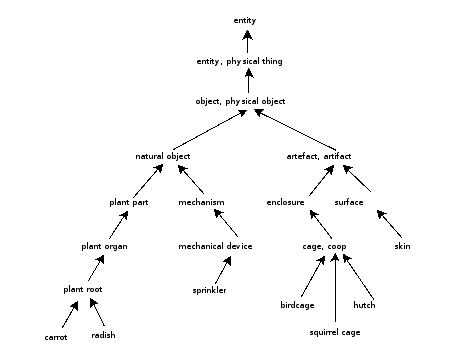
\includegraphics[width=.8\linewidth]{wordnet.png}
  \caption{WordNet directed acyclic graph. \href{http://www.cs.princeton.edu/courses/archive/spring07/cos226/assignments/wordnet.html}{Source}}
  \label{fig:wordnet}
\end{figure}
\pagebreak
The database of annotations on URLs of third-party images is freely available, but ImageNet does not own the images themselves. Since 2010, the ImageNet project has been organizing an annual competition: ImageNet Large Scale Visual Recognition Challenge (ILSVRC), or "ImageNet Large Scale Visual Recognition Competition". It consists of a software competition whose goal is to accurately detect and classify objects and scenes in natural images.

Imagenet is therefore a general classification dataset that aims to develop the vision in general, it is widely cited and widely used in many models

\pagebreak\subsection{Models}
\subsubsection{FixRes}
The top performance algorithm to date is called FixRes\cite{2019arXivFixRes}, it propose a simple but effective strategy to optimize classifier performance when train and test resolutions differ. It is only a fine adjustment of the network to the resolution of the test, inexpensive by calculation. This allows powerful classifiers to be trained using small training images. For example, FixRes achieve a top-1 accuracy of 77.1\% on ImageNet with a ResNet-50 trained on 128x128 images and 79.8\% with an image trained on 224x224 images.
Conversely, a pre-trained 32x48d ResNeXt-101 with low supervision on 940 million public images at 224x224 resolution and further optimizing the 320x320 test resolution, obtain a maximum accuracy of 86.4\% (top-5: 98.0)\%). 

FixRes is both a state of the art classification model on ImageNet\cite{pwc_classification_imagenet}, but also on iNaturalist\cite{pwc_classification_inaturalist}

\pagebreak\section{Object detection}
%https://medium.com/zylapp/review-of-deep-learning-algorithms-for-object-detection-c1f3d437b852
Object detection is locating instances of objects in images, for example, while you are looking at this text, you see multiple words next to each other, it is object detection.

Object detection models are more appropriate for identifying multiple relevant objects in a single image. The second important advantage of object detection models over image classification models is that the location of objects is provided.

\subsection{Datasets}
\subsubsection{COCO}
COCO\cite{coco} dataset is a collection of images of scenes of daily life containing common objects in their natural context (see Figure ~\ref{fig:coco}). Objects are labeled using instance-based segmentations to precise location of objects. The data set contains photos of 91 types of objects that are \begin{it}"easily recognizable by a 4-year-old child"\end{it}. With a 2.5 million instances tagged in 328,000 images.

COCO is widely used for object detection and image segmentation due to its recognition simplicity.

\begin{figure}[H]
    \centering
    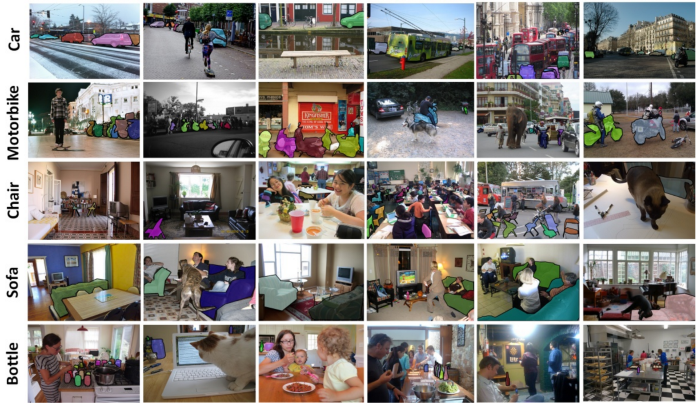
\includegraphics[scale = 0.6]{images/coco.png}
	\caption[Example COCO dataset]{Examples of segmented objects from the 2015 COCO dataset. \href{https://arxiv.org/pdf/1405.0312.pdf}{Source}}
	\label{fig:coco}
\end{figure}

\subsubsection{Open Image}
Open Image V4\cite{openimagev4} is a 9.2 million pixel image data set with unified annotations for image classification, object detection and visual relationship detection. The images have a Creative Commons Attribution license that allows you to share and adapt the material. They were collected from Flickr without a predefined list of class names or tags, thus generating natural class statistics and avoiding initial design bias. Open Images V4 offers a large scale in several dimensions: 30.1 million pixel image level labels for 19.8 KB concepts, 15.4 million pixel selection boxes for 600 object classes and 375,000 pixel visual relationship annotations for 57 classes. For object detection in particular, 15 times more enclosures is provided than the next largest datasets (15.4 million enclosures out of 1.9 million images). Images often show complex scenes with several objects (8 objects annotated per image on average). Visual relationships are annotated together, which support the detection of visual relationships, an emerging task that requires structured reasoning. Complete and detailed statistics on the dataset are provided, the quality of annotations are validated and the performance of many modern models evolution with increasing amounts of training data are delivered.

Open Image bring high quality images and is more complex for recognition than COCO, it also allow vision relationship detection.


\pagebreak\subsection{Models}
\subsubsection{Performance metrics}
\paragraph{Intersection on Union (IoU)}
IoU is a measure based on Jaccard Index that evaluates the overlap between two bounding boxes. It requires a ground truth bounding box \begin{math}B_{gt}\end{math} and a predicted bounding box \begin{math}B_{p}\end{math}. 
By applying the IoU we can tell if a detection is valid (True Positive) or not (False Positive).
IoU is given by the overlapping area between the predicted bounding box and the ground truth bounding box divided by the area of union between them: 
\begin{gather*}
\centering
\mathrm{IoU}=\frac{\operatorname{area}\left(B_{p} \cap B_{g t}\right)}{\operatorname{area}\left(B_{p} \cup B_{g t}\right)}
\end{gather*}

IoU is a value between 0 and 1, which corresponds to the overlap zone between the predicted zone and the truth zone on the ground. The higher the IoU value, the better the intended location of the box for a given object. Usually, we keep all candidates in the bounding box with an IoU above a threshold.

\pagebreak\paragraph{mean Average Precision (mAP)}

A common metric which is used for the Pascal VOC object recognition challenge is to measure the Average Precision (AP) for each class. The following description of Average Precision is taken from Everingham et. al.\footnote{\href{http://homepages.inf.ed.ac.uk/ckiw/postscript/ijcv_voc09.pdf}{Source}}

\begin{it}
The mean Average Precision (mAP) is computed by taking the average over the APs of all classes.
For a given task and class, the precision/recall curve is computed from a method’s ranked output. Recall is defined as the proportion of all positive examples ranked above a given rank. Precision is the proportion of all examples above that rank which are from the positive class. The AP summarizes the shape of the precision/recall curve, and is defined as the mean precision at a set of eleven equally spaced recall levels [0,0.1, . . . ,1]:
\begin{gather*}
    A P=\frac{1}{11} \sum_{r \in\{0,0,1, \ldots, 1\}} p_{i n t e r p}(r)
\end{gather*}

The precision at each recall level r is interpolated by taking the maximum precision measured for a method for which the corresponding recall exceeds r:
\begin{gather*}
    p_{\text {interp}}(r)=\max _{\tilde{r} : \tilde{r} \geq r} p(\tilde{r})
\end{gather*}

where p(˜r) is the measured precision at recall ˜r. The intention in interpolating the precision/recall curve in this way is to reduce the impact of the “wiggles” in the precision/recall curve, caused by small variations in the ranking of examples. It should be noted that to obtain a high score, a method must have precision at all levels of recall – this penalizes methods which retrieve only a subset of examples with high precision (e.g. side views of cars).
\end{it}



\pagebreak\subsubsection{Convolutional network based on the region (R-CNN)}
The region-based convolutional network is one of the main contemporary approach to object detection,
In R-CNN\cite{rcnn}, a selective search algorithm was used. Selective search is one of the generic object proposal generation methods.
\begin{enumerate}
    \item Try to detect objects
    \item Run a CNN on these objects
    \item Run the output into a SVM to classify the object and a linear regressor to adjust the box
\end{enumerate}
This approach can be expensive however because many crops are necessary, leading to significant duplicated computation from overlapping crops (see Figure ~\ref{fig:rcnn}).

\begin{figure}[H]
    \centering
    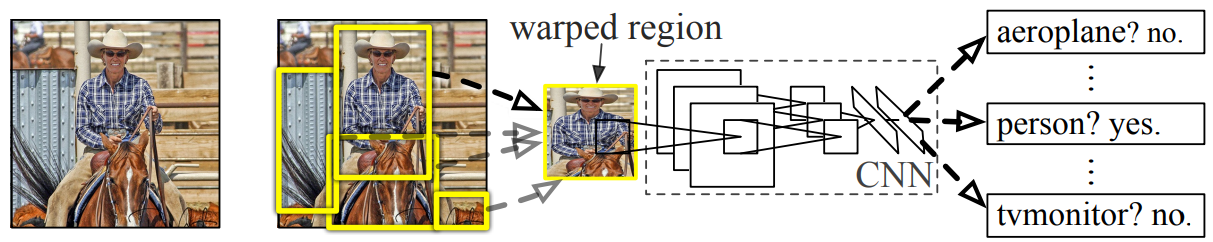
\includegraphics[scale = 0.35]{rcnn.png}
	\caption[R-CNN]{Region-based Convolution Network. (R-CNN). \href{https://arxiv.org/pdf/1311.2524v5.pdf}{Source}}
	\label{fig:rcnn}
\end{figure}


\pagebreak\subsubsection{Convolutional network based on a fast region (Fast R-CNN)}
The convolutional network based on the fast region (Fast R-CNN)\cite{fastrcnn} aims to reduce the time consumption related to the large number of models required to analyze all region proposals (see Figure ~\ref{fig:fastrcnn}).
\begin{enumerate}
    \item Performing feature extraction before proposing regions, therefore only running one CNN over the entire image instead of a CNN CNN per region
    \item Replacing the SVM with a softmax layer, therefore extending the neural network for predictions instead of creating a new model
\end{enumerate}

\begin{figure}[H]
    \centering
    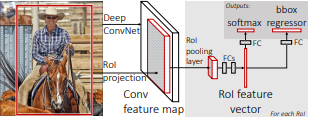
\includegraphics[scale = 0.8]{fast_rcnn.png}
	\caption[Fast R-CNN]{Region-based Convolution Network. (R-CNN). \href{https://arxiv.org/pdf/1504.08083.pdf}{Source}}
	\label{fig:fastrcnn}
\end{figure}

\pagebreak\subsubsection{Convolutional network based on faster regions (Faster R-CNN)}
The region proposals detected with the selective search method were still needed in the previous model, which is expensive in terms of calculation. 

Faster R-CNN\cite{fastrcnn} introduced the Regional Proposal Network (RPN) (see Figure ~\ref{fig:rpn}) to directly generate regional proposals, predict selection frameworks and detect objects. The convolutional network based on a faster region (Faster R-CNN) is a combination of the RPN model and the Fast R-CNN model.

\begin{enumerate}
    \item At the last layer of an initial CNN, a 3x3 sliding window moves across the feature map and maps it to a lower dimension (256-d)
    \item For each sliding-window location, it generates multiple possible regions based on k fixed-ratio anchor boxes
    \item Each region proposal consists of an “objectness” score for that region and 4 coordinates representing the bounding box of the region
\end{enumerate}


\begin{figure}[H]
    \centering
    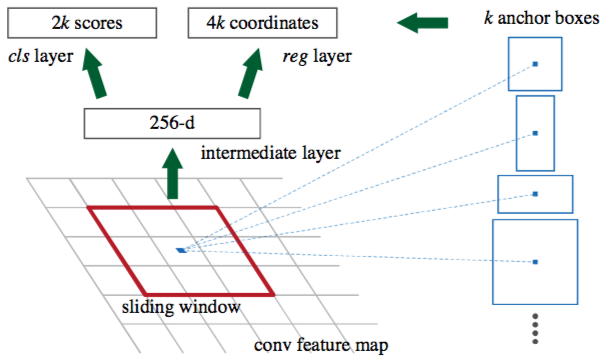
\includegraphics[scale = 0.5]{faster_rcnn.png}
	\caption[Region Proposal Network]{Region Proposal Network.  \href{https://arxiv.org/pdf/1506.01497.pdf}{Source}}
	\label{fig:rpn}
\end{figure}

The faster R-CNN uses RPN to avoid the selective search method, it speeds up training and testing processes and improves performance.

\begin{comment} % add or not
\begin{figure}[H]
    \centering
    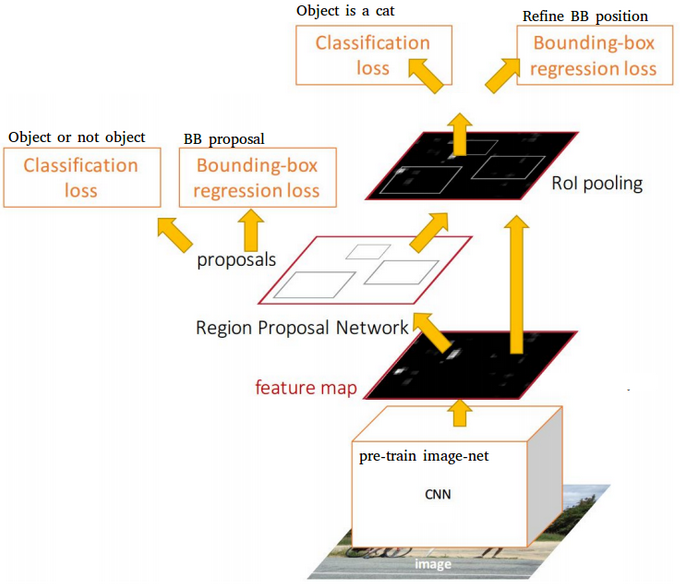
\includegraphics[scale = 0.35]{faster_rcnn2.png}
	\caption[Faster R-CNN]{Faster R-CNN = RPN + Fast R-CNN.   \href{https://arxiv.org/pdf/1506.01497.pdf}{Source}}
\end{figure}
\end{comment}


\pagebreak\subsubsection{Fully convolutional region-based network (R-FCN)}
The fast and rapid methodologies of R-CNN consist in detecting region proposals and recognizing an object in each region. The fully convolutional region-based network (R-FCN) is a model with only convolutional layers allowing to share all the computation.

R-FCN merge the two basic steps into a single model to simultaneously take into account object detection (location invariant) and its position (location variant).

\begin{enumerate}
    \item Run a CNN over the input image
    \item Add a fully convolutional layer to generate a score bank of the aforementioned “position-sensitive score maps.” There should be k²(C+1) score maps, with k² representing the number of relative positions to divide an object (e.g. 3² for a 3 by 3 grid) and C+1 representing the number of classes plus the background.
    \item Run a fully convolutional region proposal network (RPN) to generate regions of interest (RoI’s)
    \item For each RoI, divide it into sub-regions as the score maps
    \item For each sub-regions, compare with the score bank to see if it matches the corresponding position of some object.
    \item Once each of the sub-regions has an object match value for each class, average the sub-regions to get a single score per class.
    \item Classify the RoI with a softmax over the remaining C+1 dimensional vector
\end{enumerate}


\begin{figure}[H]
    \centering
    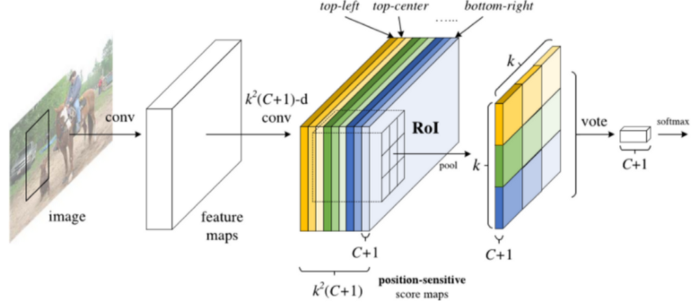
\includegraphics[scale = 0.5]{rfcn.png}
	\caption[R-FCN]{Fully convolutional region-based network. \href{https://arxiv.org/pdf/1605.06409.pdf}{Source}}
\end{figure}

In simple terms, the R-FCN examines each region proposal, dividing it into sub-regions.
For each sub-region, he asks: "Does it look like the left end of a baby?", "Does it look like the upper center of a baby?" "Does it look like a baby's top right?" etc. For all possible classes.  If enough sub-regions say "yes, I match up with a part of a baby", the RoI is classified as a baby after a softmax over all classes (see Figure ~\ref{fig:rfcnbaby}).


\begin{figure}[H]
    \centering
    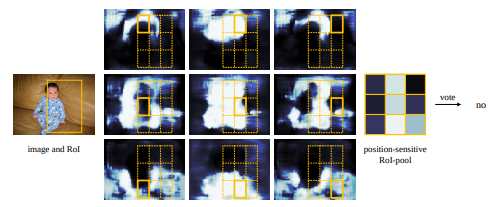
\includegraphics[scale = 0.7]{rfcn2.png}
	\caption[R-FCN2]{Visualization of R-FCN (k × k = 3 × 3) for the person category.  \href{https://arxiv.org/pdf/1605.06409.pdf}{Source}}
	\label{fig:rfcnbaby}
\end{figure}

\begin{figure}[H]
    \centering
    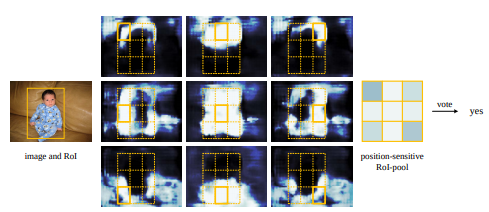
\includegraphics[scale = 0.7]{rfcn3.png}
	\caption[R-FCN3]{Visualization when an RoI does not correctly overlap the object.  \href{https://arxiv.org/pdf/1605.06409.pdf}{Source}}
\end{figure}



\pagebreak\subsubsection{You only look once (YOLO)}
The YOLO\cite{yolo} model directly predicts bounding boxes and class probabilities with a single network in a single assessment. The simplicity of the YOLO model allows real-time predictions.
YOLO is doing an end-to-end learning paradigm: proposals, features, and the classifier becoming one neural network (see Figure ~\ref{fig:yolo}). 

One indispensable component is non-maximum suppression (NMS), a post-processing algorithm responsible for merging all detections that belong to the same object. 

\begin{enumerate}
    \item Split our image into cells. Each cell will be responsible for predicting bounding boxes score, this score is simply the probability to detect the object multiplied by the IoU between the predicted and the ground truth boxes.
    \item Remove boxes with low object probability and bounding boxes with the highest shared area in the process called non-max suppression.
\end{enumerate}


\begin{figure}[H]
    \centering
    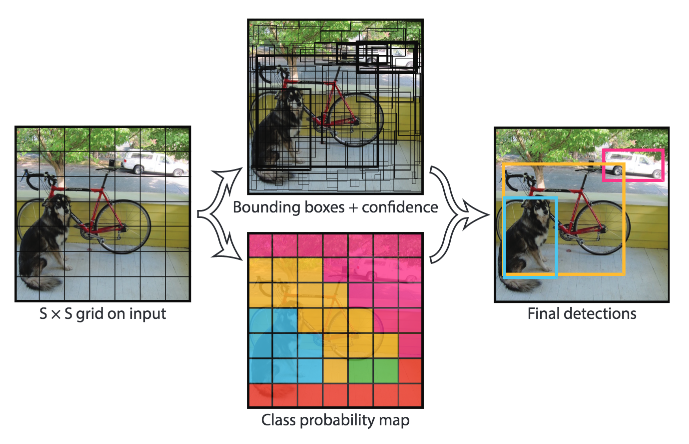
\includegraphics[scale = 0.5]{yolo.png}
	\caption[YOLO]{Imaged example of the steps of YOLO. \href{https://arxiv.org/pdf/1506.02640.pdf}{Source}}
	\label{fig:yolo}
\end{figure}

\begin{comment}
\begin{figure}[H]
    \centering
    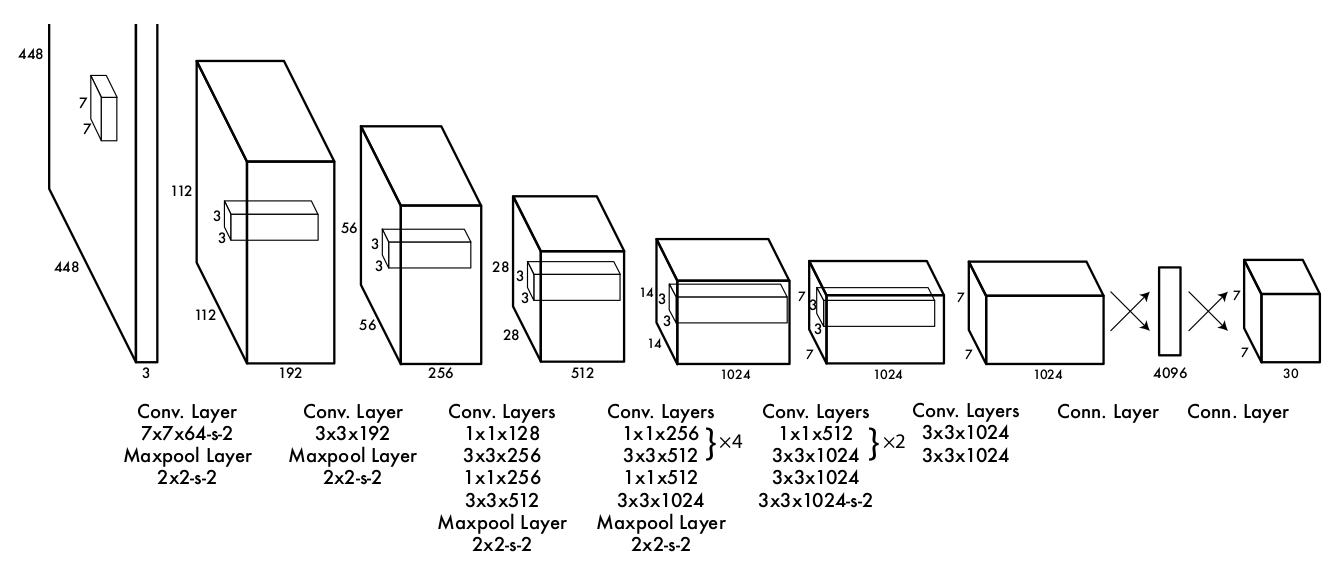
\includegraphics[scale = 0.20]{yolo2.png}
	\caption[YOLO2]{YOLO architecture \href{https://arxiv.org/pdf/1506.02640.pdf}{Source}}
\end{figure}
\end{comment}


\pagebreak\subsubsection{Single-shot detector (SSD)}
Similar to the YOLO model, Single Shot Detector (SSD)\cite{ssd} predict both bounding boxes and class probabilities with an end-to-end CNN architecture (see Figure ~\ref{fig:ssdyolo}).

The SSD model uses extra feature layers from different feature maps of the network in order to increase the number of relevant bounding boxes.

\begin{enumerate}
    \item The model takes as input an image that passes through several convolution layers with different filter sizes (10x10, 5x5 and 3x3) that will generate feature maps.
    \item Each location in these feature maps are processed by specific convolution layers with 3x3 filters, to produce a set of bounding boxes similar to the Fast R-CNN anchor boxes.
    \item For each box, simultaneously predict the bounding box location and the class probabilities.
    \item During training, match the ground truth box with these predicted boxes based on IoU. The best predicted box will be labeled a “positive,” along with all other boxes that have an IoU with the truth > 0.5.
\end{enumerate}



\begin{figure}[H]
    \centering
    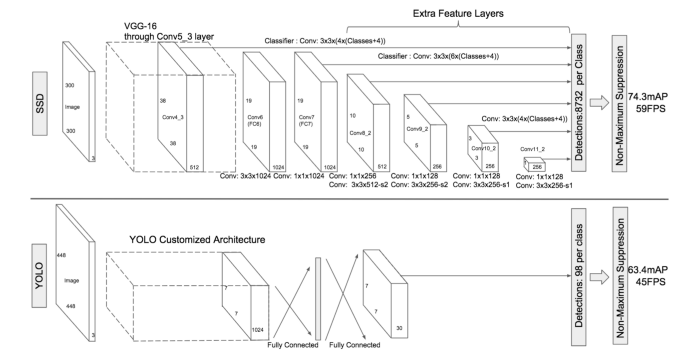
\includegraphics[scale = 0.5]{ssd.png}
	\caption[SSD]{Comparison between the SSD and the YOLO architectures. \href{https://arxiv.org/pdf/1512.02325.pdf}{Source}}
	\label{fig:ssdyolo}
\end{figure}
\pagebreak
The varying-size feature maps brought by SSD help capture objects of different sizes. Here is an example of SSD inference (see Figure ~\ref{fig:ssdinf}).

\begin{figure}[H]
    \centering
    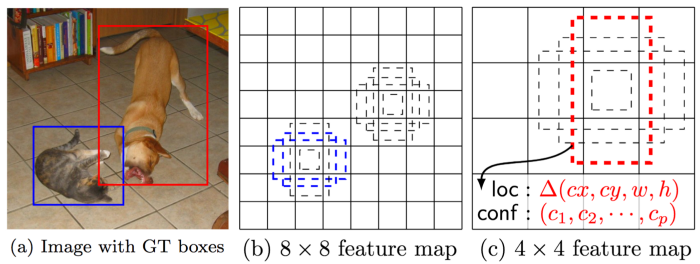
\includegraphics[scale = 0.5]{ssd2.png}
	\caption[SSD2]{SSD Framework. \href{https://arxiv.org/pdf/1512.02325.pdf}{Source}}
	\label{fig:ssdinf}
\end{figure}

In the end SSD does two things:
\begin{itemize}
    \item First, apply non-maximum suppression to group boxes that overlap strongly. In other words, if four boxes of similar shapes, sizes, etc. contain the same cat, NMS will keep the one with the most confidence and reject the rest. 
    \item Second, the model uses a technique called hard negative mining to balance classes during training. In the case of hard negative mining, only a subset of the negative examples with the highest training loss (i.e. false positives) are used for each iteration of the training. SSD maintains a 3:1 ratio between negatives and positives.
\end{itemize}

\pagebreak\subsubsection{Neural Architecture Research Network (NASNet)}

NASNet\cite{nasnet} consists in learning the architecture of a model using reinforcement learning to optimize the number of layers while improving the accuracy of a given data set. NASNet achieved superior performance with a lighter model than previous work compared to the 2012 ImageNet classification challenge (see Figure ~\ref{fig:nasnet}).
The NASNet network has an architecture learned from the CIFAR-10\cite{cifar10} dataset and is trained in the ImageNet 2012 dataset.

From the official paper:

\begin{it}
"Our approach is inspired by the recently proposed Neural Architecture Search (NAS) framework, which uses a reinforcement learning search method to optimize architecture configurations. Applying NAS, or any other search methods, directly to a large dataset, such as the ImageNet dataset, is however computationally expensive. We therefore propose to search for a good architecture on a proxy dataset, for example the smaller CIFAR-10 dataset, and then transfer the learned architecture to ImageNet."
\end{it}

\begin{figure}[H]
    \centering
    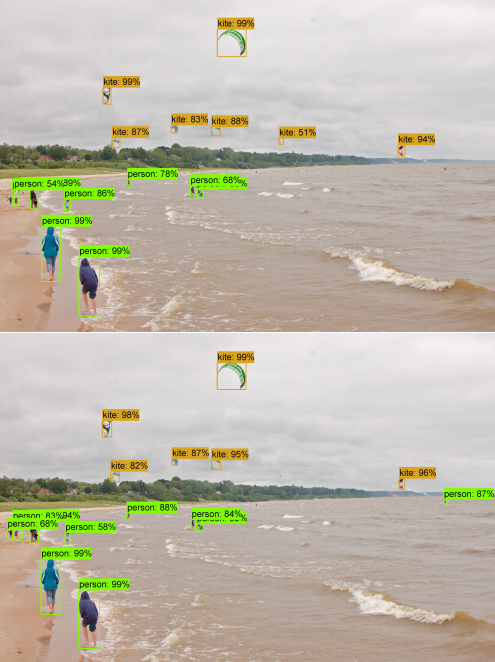
\includegraphics[scale = 0.4]{nasnet.png}
	\caption[NASNet]{Example of object detection results differences between Faster-RCNN
    with Inception-ResNet-v2 featurization (top) and NASNet-A featurization (bottom). \href{https://arxiv.org/pdf/1707.07012.pdf}{Source}}
    \label{fig:nasnet}
\end{figure}

\pagebreak\subsubsection{Convolutional network based on a mask region (Mask R-CNN)}
Mask R-CNN\cite{maskrcnn} is an extension over Faster R-CNN. Faster R-CNN predicts bounding boxes and Mask R-CNN essentially adds one more branch for predicting an object mask in parallel (see example on Figure ~\ref{fig:maskrcnn}).

\begin{figure}[H]
    \centering
    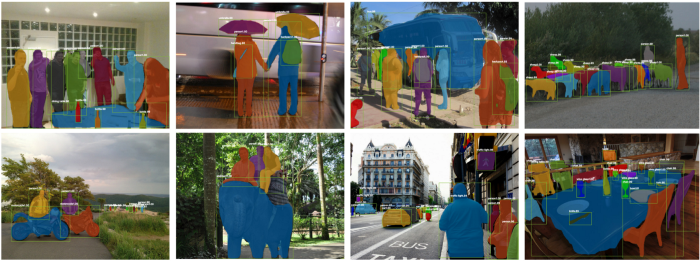
\includegraphics[scale = 0.5]{mask_rcnn.png}
	\caption[Mask R-CNN2]{Examples of Mask R-CNN application on the COCO test dataset.  \href{https://arxiv.org/pdf/1703.06870.pdf}{Source}}
	\label{fig:maskrcnn}
\end{figure}

There are two stages of Mask R-CNN (see Figure ~\ref{fig:maskrcnn2}). 
\begin{enumerate}
    \item Generates proposals about the regions where there might be an object based on the input image.
    \item Predicts the class of the object, refines the bounding box and generates a mask in pixel level of the object based on the first stage proposal. Both stages are connected to the backbone structure.
\end{enumerate}

\begin{it}
"The mask branch is a small FCN applied to each RoI, predicting a segmentation mask in a pixel-to-pixel manner."\cite{maskrcnn}
\end{it}

\begin{figure}[H]
    \centering
    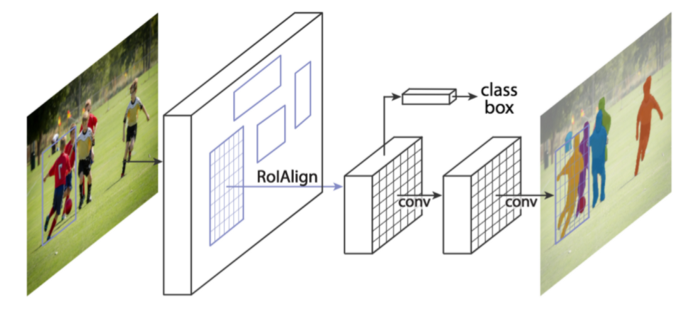
\includegraphics[scale = 0.5]{mask_rcnn2.png}
	\caption[Mask R-CNN2]{Mask R-CNN framework for instance segmentation. \href{https://arxiv.org/pdf/1703.06870.pdf}{Source}}
	\label{fig:maskrcnn2}
\end{figure}

\pagebreak\subsection{Object detection conclusion}
Over the years, object detection models tend to infer that location and classification have a fully differentiable network. Therefore, it can be trained from head to tail with neural networks in a end-to-end manner.

The most important question is not which detector is the best. It may not be possible to answer. The real question is which detector and which configurations offer us the best balance between speed and accuracy that your application needed. Below is a comparison of the accuracy vs speed tradeoff (time measured in milliseconds) (see Figure ~\ref{fig:odbenchmark}).

\begin{figure}[H]
    \centering
    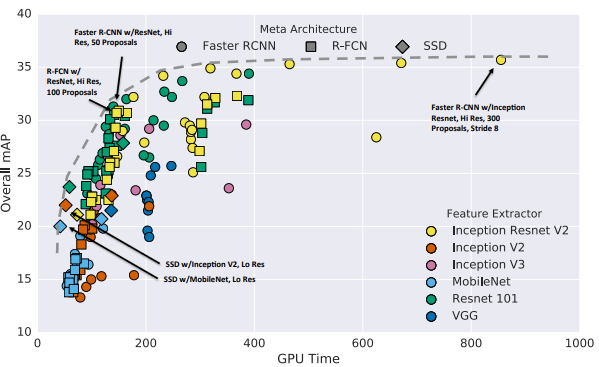
\includegraphics[scale = 0.7]{object_detection_benchmark.png}
	\caption{Object detection speed vs accuracy tradeoff. \href{https://arxiv.org/pdf/1611.10012.pdf}{Source}}
	\label{fig:odbenchmark}
\end{figure}

\pagebreak\section{Action classification}

Learning to understand videos is a very difficult task, both in terms of algorithms and calculations, the networks have access to not only the appearance information present in single, static images, but also their complex temporal evolution. 
Such a task could be useful to analyse wildlife behaviours, a kind of information that is very rare.

\subsection{Datasets}

\subsubsection{Charades}
Charades-Ego\cite{charades} is a 68,536 instances of activity in 68.8 hours of first and third person video, making it one of the largest and most diverse egocentric data sets in the world. Charades-Ego also shares activity classes, scripts and methodology with the Charades data set, which consists of an additional 82.3 hours of third person video with 66,500 activity instances. Charades-Ego has time annotations and text descriptions, making it suitable for self-centered video classification, localization, subtitling and new tasks using the inter-modal nature of data.

\subsubsection{Moments in Time}
Moments in Time\cite{momentsintime} dataset is a large-scale collection of one million short videos, annotated by man, corresponding to dynamic events taking place in less than three seconds. Modelling spatio-temporal dynamics, even for actions made in 3-second videos, poses many challenges: significant events include not only people, but also objects, animals and natural phenomena; visual and auditory events can be time-symmetric ("opening" is "closing" in the opposite direction) and transient or prolonged. The annotation process (each video is labelled with an action or activity label among 339 different classes), analyze its scale and diversity compared to other large-scale video data sets for action recognition, and present the results of several basic models. treat separately and jointly three modalities: spatial, temporal and auditory. The Moments in Time dataset, designed to cover many visual and auditory events and a wide variety of events, can be a new challenge in developing models that adapt to the level of complexity and abstract reasoning that a human deals with on a daily basis.

\pagebreak\subsection{Models}
\subsubsection{AssembleNet}
Standard CNN video CNN architectures have been designed by directly extending architectures designed for image understanding to a third dimension (using a limited number of spatio-temporal modules such as 3D convolutions) or by introducing a handmade two-stream design to capture both appearance and motion in videos. AssembleNet\cite{assemblenet} interpret a video CNN as a collection of multi-flow space-time convolution blocks connected to each other, and propose the approach of automatically searching for neural architectures with better connectivity for video comprehension. This is done by developing a population of overly connected architectures guided by learning the connection weight. Architectures combining representations that do not have different types of input (i.e. RGB and optical flow) at multiple temporal resolutions are sought, thus allowing different types or sources of information to interact. AssembleNet, surpasses previous approaches to public video data sets, in some cases with a large margin.

\pagebreak\section{Visual object tracking}

Visual object tracking is an interesting task that could also help to understand the species behaviour, for example if you can see on large amount of data that certain animal often goes into a certain direction ...

\subsection{Datasets}
\subsubsection{VOT}
The VOT2018\cite{vot2018} Challenge, followed by visual objects, is the sixth annual comparative analysis of monitoring organized by the VOT initiative. The results of more than 80 trackers are presented; many are leading trackers published at major computer vision conferences or in journals in recent years. The evaluation included the standard VOT method and other popular short-term follow-up analysis methods and a "real time" experiment simulating a situation in which a tracker treats images as if they were provided by a continuously operating sensor. A long-term monitoring sub-challenge has been introduced for all standard VOT sub-challenges. The new sub-challenge addresses the long-term monitoring properties, namely the management of target disappearance and reappearance. A new data set has been compiled and a performance evaluation methodology focusing on long-term monitoring capacities has been adopted. The VOT toolbox has been updated to support standard and long-term short-term monitoring sub-challenges. The performance of the follow-ups tested generally far exceeds the standard reference levels.

\pagebreak\subsection{Models}
\subsubsection{THOR}
Currently, the state-of-the-art algorithm to date on the VOT challenge is called thor\cite{thor}:

This algorithm focus on the construction of holistic object representations for tracking. The structure exploits the idea of obtaining additional object models during the tracking process. The resulting representation contains information beyond the location of the truth object on the ground provided to the system. It is then useful for orientation, but also for other tasks requiring a visual understanding of objects. Strong empirical results on monitoring benchmarks indicate that the method can improve the performance and robustness of underlying monitoring while reducing its speed. In addition, the method is able to reproduce current results, while using a simpler and older network architecture and operating three times faster.


\pagebreak\section{Wild life}

During the past decades, engineers and wildlife researchers have developed various hardware technologies for professionals to monitor individual mammals,
including very high frequency (VHF) radio tracking\cite{radio1983}\cite{inradio}\cite{satellite2018}, 
and Global Positioning System (GPS) tracking \cite{zebranet2002}\cite{gps2001}\cite{kruger2016inexpensive},
wireless sensor networks\cite{sensornet2002}\cite{sensornet2004},  
animal-mounted video monitoring systems \cite{portablecamera2008}, 
drones to captures images from above\cite{s16010097} and ultimately motion-triggered cameras which are useful to capture images only when an animal is present and in his natural environment including at night thanks to infrared.


A motion-triggered camera is a camera with an automatic gesture detection system, which activates the shot as soon as the sensor detects a movement (see example on Figure ~\ref{fig:camtrap}). 
Its continuous image analysis operation is similar to the proximity sensor with the additional capabilities to be transported, adapt to a medium, record and process images.

\begin{figure}[H]
\centering
\begin{subfigure}{.5\textwidth}
  \centering
  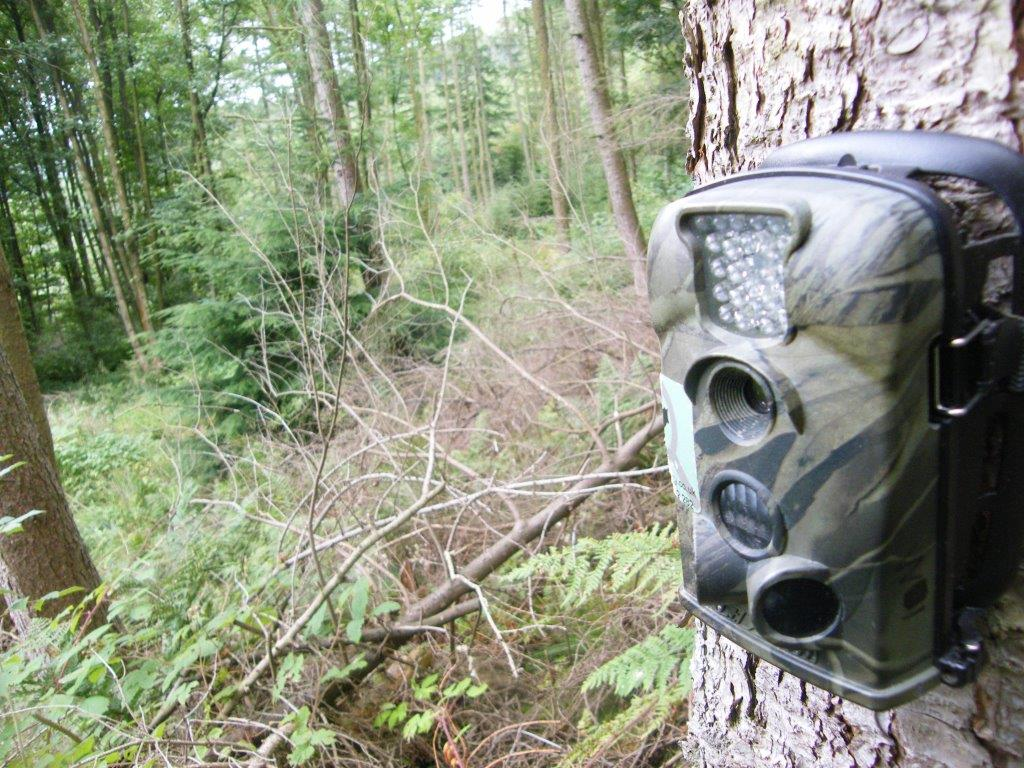
\includegraphics[width=.8\linewidth]{camera_trap.jpg}
  \caption{Camera trap. \href{https://shop.naturespy.org/wp-content/uploads/2014/05/Ltl-Acorn-camera-trap-1.jpg}{Source}}
\end{subfigure}%
\begin{subfigure}{.5\textwidth}
  \centering
  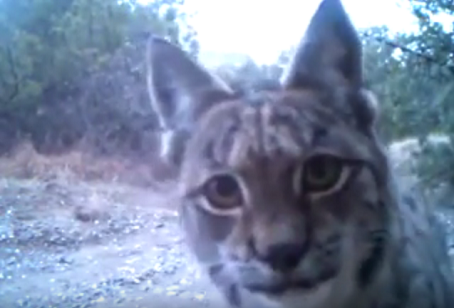
\includegraphics[width=.8\linewidth]{lynx.png}
  \caption{Lynx taken by camera trap. \href{https://agenda.ge/en/news/2015/2337}{Source}}
\end{subfigure}
\caption{Camera trap \& Picture taken by it}
\label{fig:camtrap}
\end{figure}

\pagebreak\subsection{Datasets}

\subsubsection{iNaturalist}
iNaturalist is a citizen science project and an online social network of naturalists, citizen scientists and biologists based on the concept of mapping and sharing biodiversity observations around the world. iNaturalist is accessible through its website or mobile applications. Observations recorded with iNaturalist provide valuable open data for scientific research projects, conservation agencies, other organizations and the public. The project has been described as "flagship for mobile natural history applications.
The dataset consists of 859,000 images from over 5,000 different species of plants and animals.
iNaturalist is different from camera trap datasets, it is probably between camera trap and ImageNet-like dataset since it is taken by amateurs.

\subsubsection{iWildCam 2018 Challenge Dataset}
iWildCam\cite{iwildcam2019} consists of 292,732 images on 143 locations in American SouthWest, each labelled either as containing an animal or as empty.

iWildCam is also a challenge in which training data and test data come from different regions. The species observed in each region overlap, but are not identical.

iWildCam 2018 is the biggest public camera-trap dataset for southwest wildlife.

\subsubsection{North American Camera Trap Images}
This data set\cite{north_american_camera_trap_and_resnet18} contains 3.7 million photographic trap images from five different locations in the United States, with tags for 28 animal categories, mainly at the species level (for example, the most common tags are cattle, boars and deer). About 12\% of the images are labelled as empty.
North American Camera Trap Images is the biggest public camera-trap dataset for north American wildlife


\pagebreak\subsubsection{Snapshot Seregenti}
Hundreds of camera traps in Tanzania's Serengeti National Park open a powerful new window into the dynamics of Africa's most elusive wildlife species. The camera traps have been in continuous operation since 2010 and has produced millions of images, classified by volunteers.

This data set contains approximately 2.5 million camera trap image sequences, for a total of 6.7 million images, from seasons one to ten of the Snapshot Serengeti project. Tags are provided for 55 animal categories, mainly at the species level (for example, the most common tags are wildebeest, zebra and Thomson's gazelle). About 75\% of the images are labelled as empty. There is approximately 150,000 selection box annotations to approximately 78,000 of these images.

Snapshot Seregenti is surely the biggest public camera-trap dataset for African wildlife.

\pagebreak\subsubsection{Synthetic data}
Synthetic data and simulated environment are really promising, the advances in the field of computer graphics enable the modeling of 3D world looking closely to reality and can be generated infinitely.
Airsim\cite{airsim} is an open source system designed to form autonomous systems. AirSim provides realistic environments, vehicle dynamics and multimodal detection to researchers who build autonomous vehicles using AI to improve their safe operation in an open world.

Engineers who build autonomous systems can create accurate and detailed models of systems and environments, making them intelligent using methods such as in-depth learning, imitation learning and reinforcement learning. Tools such as Bonsai can be used to train models for a variety of environmental conditions and vehicle scenarios in the cloud on Microsoft Azure - much faster and safer than what is feasible in the real world. Once the training is complete, designers can deploy these trained models on real hardware.
Airsim has evolved towards a general purpose simulated environment and now contains also wildlife and camera-traps (see Figure ~\ref{fig:airsim}).

\begin{figure}[H]
\centering
\begin{subfigure}{.5\textwidth}
  \centering
  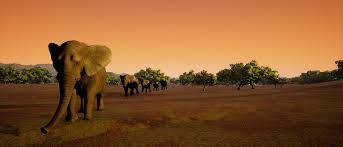
\includegraphics[width=.8\linewidth]{airsim_elephant.jpeg}
  \caption{Airsim elephant. \href{http://teamcore.usc.edu/papers/2018/bondi_camera_ready_airsim-w.pdf}{Source}}
\end{subfigure}%
\begin{subfigure}{.5\textwidth}
  \centering
  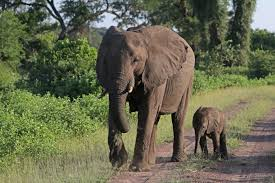
\includegraphics[width=.8\linewidth]{real_elephant.jpeg}
  \caption{Real elephant. \href{https://commons.wikimedia.org/wiki/User:Charlesjsharp/favourites}{Source}}
\end{subfigure}
\caption{Example showing differences between synthetic and real animal}
\label{fig:airsim}
\end{figure}

Synthetic data are still far from real data but it can still be used to learn the general pattern of specific data, the advantage is that synthetic data are unlimited.

\pagebreak\subsection{Models}

In the case of camera-trap images, we can't simply directly use the same models that has been trained on animal images taken by professionals.
Motion triggered camera images have lower quality and are highly cluttered with low contrast, and with dramatic background motion. Pattern detection also needs to handle a wide variety of animal body sizes, appearance, and poses (see differences example in Figure ~\ref{fig:camtraprealcam}).

\begin{figure}[H]
\centering
\begin{subfigure}{.5\textwidth}
  \centering
  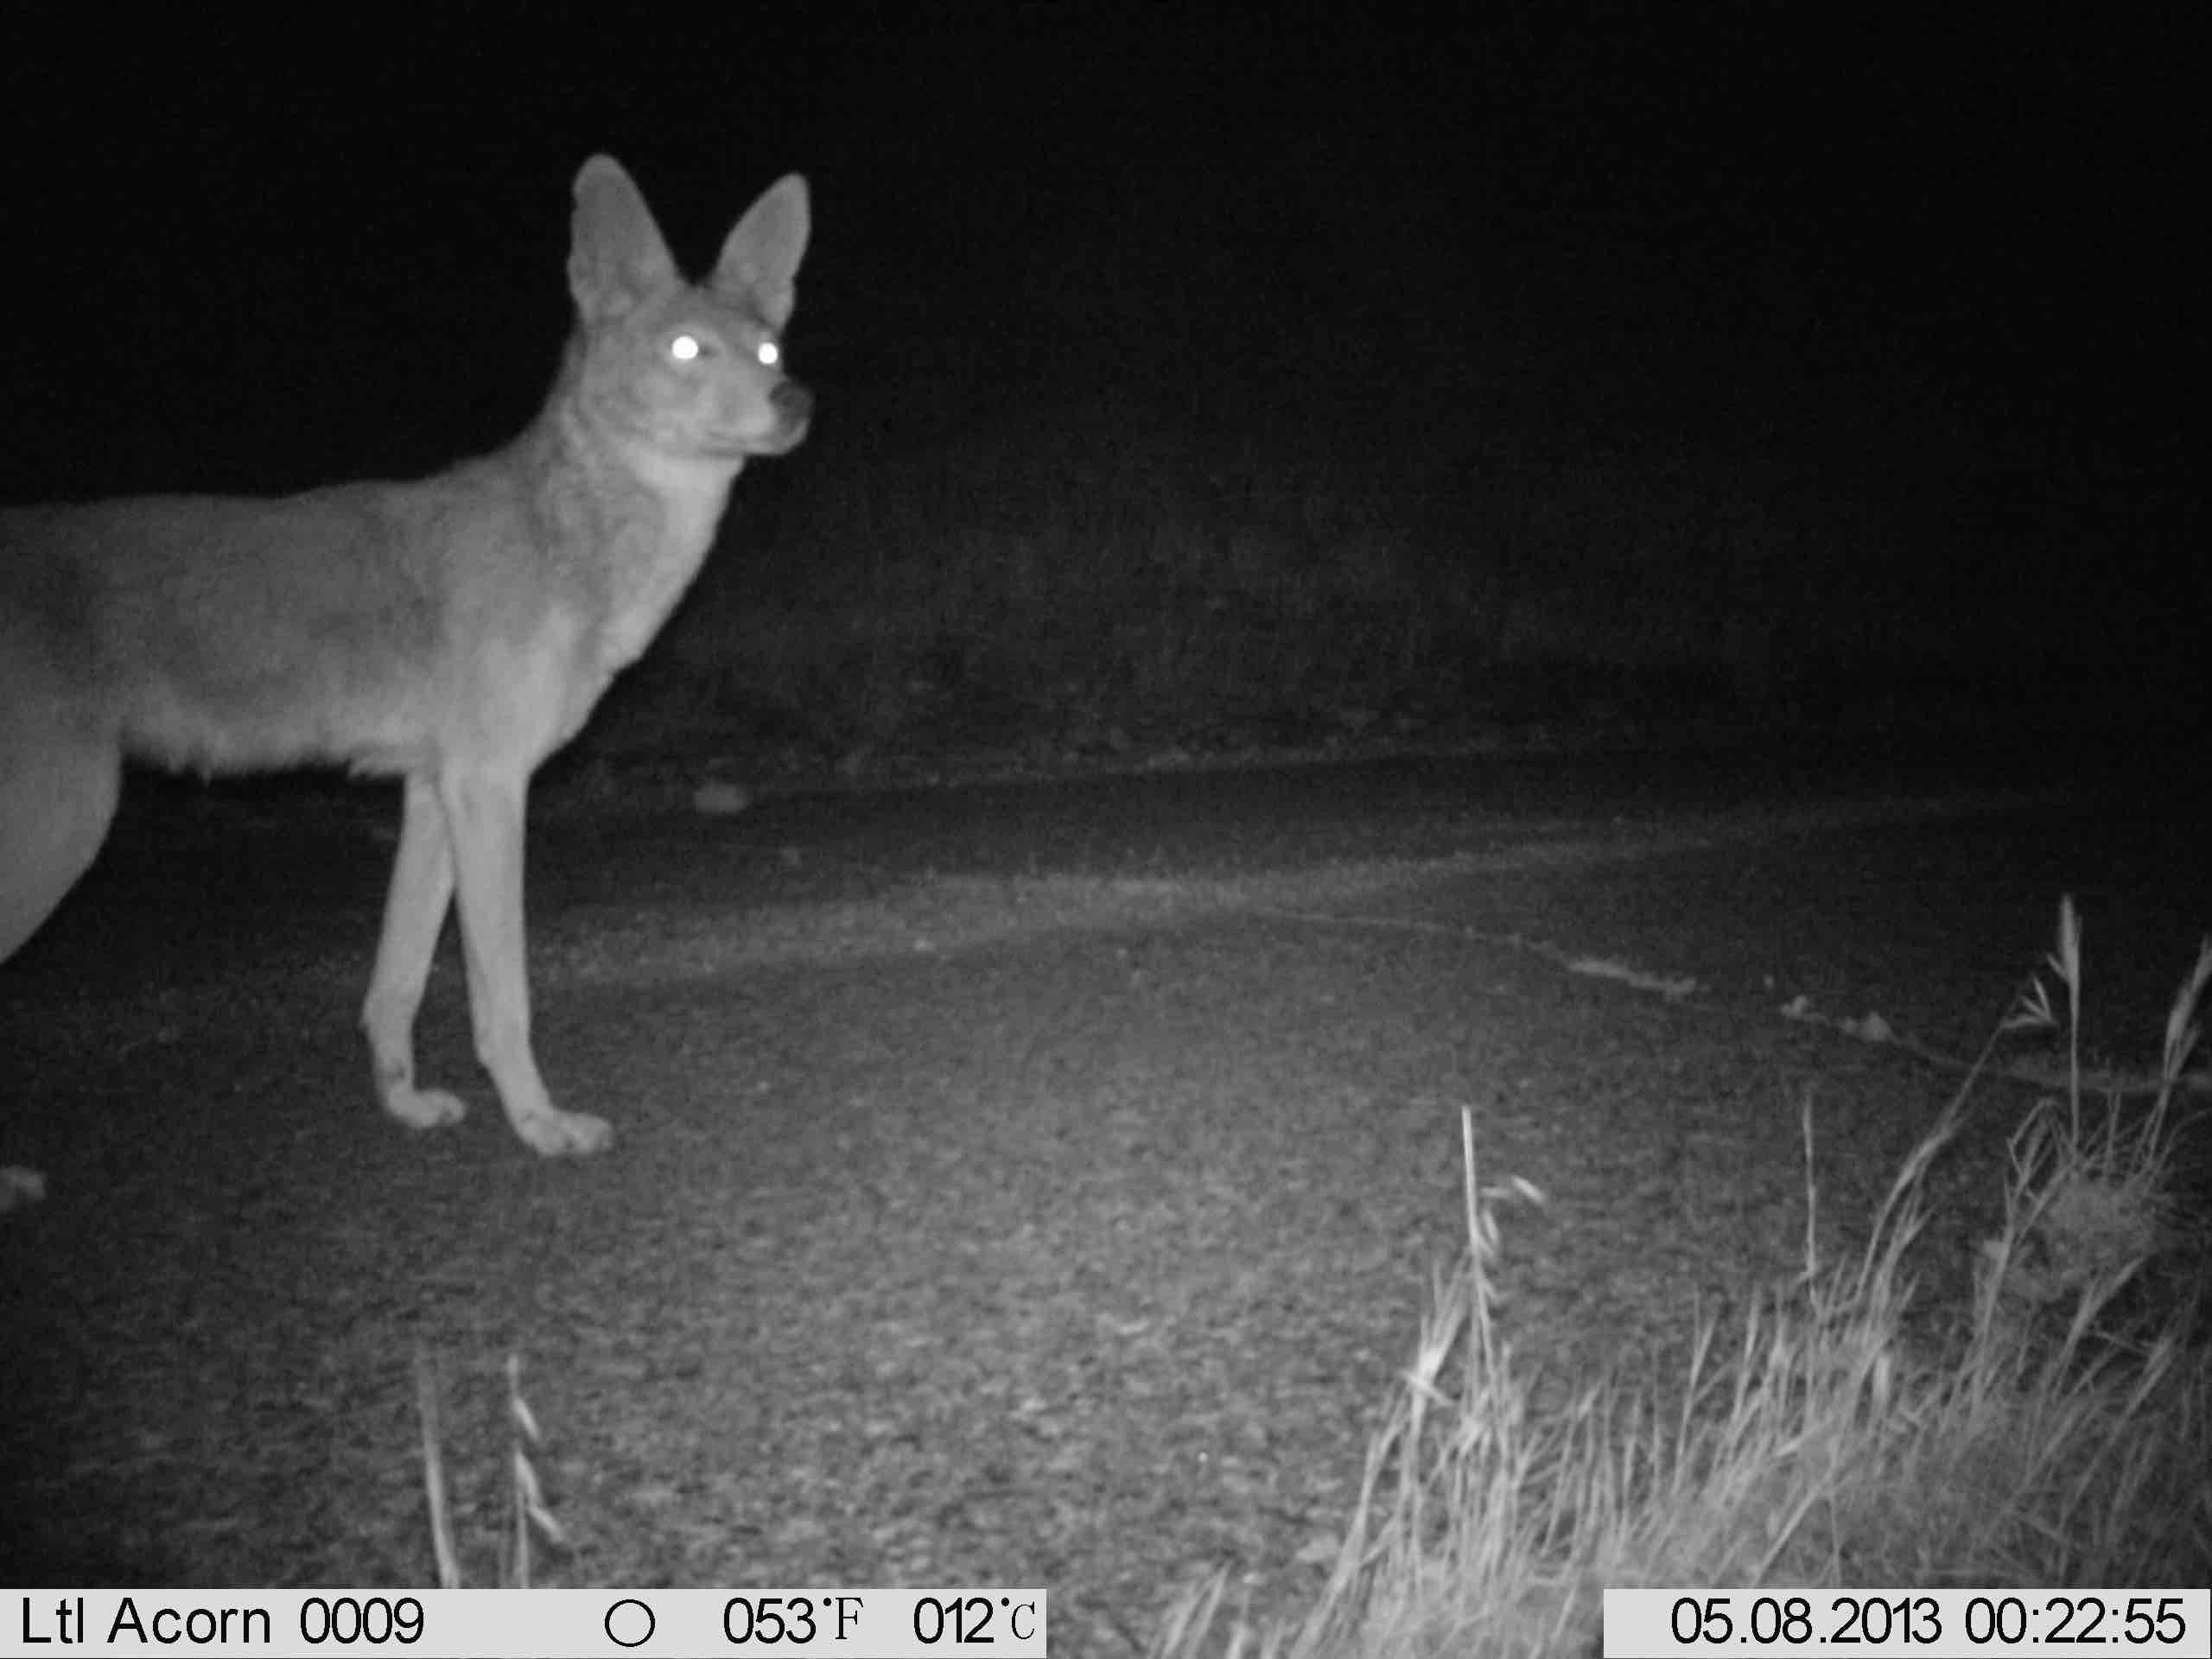
\includegraphics[width=.8\linewidth]{iwildcam_sample.jpg}
  \caption{Camera-trap sample}
\end{subfigure}%
\begin{subfigure}{.5\textwidth}
  \centering
  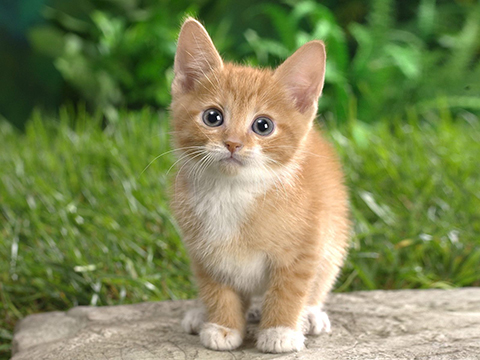
\includegraphics[width=.8\linewidth]{imagenet_sample.jpg}
  \caption{ImageNet sample}
\end{subfigure}
\caption[Camera-trap vs professional photography]{Example showing the differences between camera-trap image and professional photograph quality image}
\label{fig:camtraprealcam}
\end{figure}

Often, the images taken by camera trap are not free of right, causing a huge difference in quantity of publicly available datasets compared to general images datasets.

Transfer learning is an interesting solution when there is a lack of the specific data we want to train on.
Used by many\cite{feature_learning_bengio}\cite{decaf_feature}\cite{transfer_learning_bengio}\cite{dl__imagenet_seregenti_gomez}\cite{dl_imagenet_seregenti_norouzzadeh}, usually pre-training a model with ImageNet or similar general dataset then fine tuning with camera trap datasets like iWildcam and such.

\pagebreak\section{Conclusion}

Classification and detection are useful for wildlife monitoring, but action classification and other "exotic" tasks may be interesting in the future.
The advantage of object detection over classification is to know the position of the objects as well as to have several results per image, that's why I chose to focus on detection in the rest of this work